%%%%%%%%%%%%%%%%%%%%%%%%%%%%%%%%%%%%%%%%%
% Template de Relatório
% Version 0.8 (12/04/19)
%
% Authors:
% Franklin Coêlho
% Eudisley Anjos
% 
% License:
% CC BY-NC-SA 3.0 (http://creativecommons.org/licenses/by-nc-sa/3.0/)
%%%%%%%%%%%%%%%%%%%%%%%%%%%%%%%%%%%%%%%%%

\documentclass[10pt, a4paper, twocolumn]{article} 

%%%%%%%%%%%%%%%%%%%%%%%%%%%%%%%%%%%%%%%%%
% Wenneker Article
% Structure Specification File
% Version 1.0 (28/2/17)
%
% This file originates from:
% http://www.LaTeXTemplates.com
%
% Original Authors:
% Frits Wenneker
% Vel (vel@LaTeXTemplates.com)
%
% Adaptation:
% Frankin Coêlho (franklinanthony@eng.ci.ufpb.br)
% Eudisley Anjos (eudisley@ci.ufpb.br)
%
% License:
% CC BY-NC-SA 3.0 (http://creativecommons.org/licenses/by-nc-sa/3.0/)
%
%%%%%%%%%%%%%%%%%%%%%%%%%%%%%%%%%%%%%%%%%

%----------------------------------------------------------------------------------------
%	PACKAGES AND OTHER DOCUMENT CONFIGURATIONS
%----------------------------------------------------------------------------------------

% CI logo colors

\usepackage[english]{babel} % English language hyphenation

%\usepackage{authblk}} %Added by Eudis

\usepackage{microtype} % Better typography

\usepackage{amsmath,amsfonts,amsthm,bm} % Math packages for equations

\usepackage[svgnames]{xcolor} % Enabling colors by their 'svgnames'
\definecolor{blueCI}{rgb}{0.0, 0.2, 0.4}
\definecolor{blackCI}{rgb}{0.086, 0.13,0.16}

\usepackage[hang, small, labelfont=bf, up, textfont=it]{caption} % Custom captions under/above tables and figures

\usepackage{booktabs} % Horizontal rules in tables

\usepackage{lastpage} % Used to determine the number of pages in the document (for "Page X of Total")

\usepackage{graphicx} % Required for adding images

\usepackage{enumitem} % Required for customising lists
\setlist{noitemsep} % Remove spacing between bullet/numbered list elements

\usepackage{sectsty} % Enables custom section titles
\allsectionsfont{\color{blackCI}} % Change the font of all section commands (Helvetica)

\usepackage[colorlinks,linkcolor=blueCI,urlcolor=blueCI,citecolor=blueCI]{hyperref}
\urlstyle{same} % same font as text

\usepackage{lipsum}

%----------------------------------------------------------------------------------------
%	MARGINS AND SPACING
%----------------------------------------------------------------------------------------

\usepackage{geometry} % Required for adjusting page dimensions

\geometry{
	top=1cm, % Top margin
	bottom=1.5cm, % Bottom margin
	left=2cm, % Left margin
	right=2cm, % Right margin
	includehead, % Include space for a header
	includefoot, % Include space for a footer
	%showframe, % Uncomment to show how the type block is set on the page
}

\setlength{\columnsep}{7mm} % Column separation width

%----------------------------------------------------------------------------------------
%	FONTS
%----------------------------------------------------------------------------------------

\usepackage[T1]{fontenc} % Output font encoding for international characters
\usepackage[utf8]{inputenc} % Required for inputting international characters

\usepackage[sfdefault,scaled=.85]{FiraSans}
\usepackage{newtxsf}
%----------------------------------------------------------------------------------------
%	HEADERS AND FOOTERS
%----------------------------------------------------------------------------------------

\usepackage{fancyhdr} % Needed to define custom headers/footers
\pagestyle{fancy} % Enables the custom headers/footers

\renewcommand{\headrulewidth}{0.0pt} % No header rule
\renewcommand{\footrulewidth}{0.4pt} % Thin footer rule

\renewcommand{\sectionmark}[1]{\markboth{#1}{}} % Removes the section number from the header when \leftmark is used

%\nouppercase\leftmark % Add this to one of the lines below if you want a section title in the header/footer

% Headers
\lhead{} % Left header
\chead{\textit{\thetitle}} % Center header - currently printing the article title
\rhead{} % Right header

% Footers
\lfoot{} % Left footer
\cfoot{} % Center footer
\rfoot{\footnotesize \thepage}% de \pageref*{LastPage}} % Right footer, "Page 1 of 2"

\fancypagestyle{firstpage}{ % Page style for the first page with the title
	\fancyhf{}
	\renewcommand{\footrulewidth}{0pt} % Suppress footer rule
}

%----------------------------------------------------------------------------------------
%	TITLE SECTION
%----------------------------------------------------------------------------------------

\newcommand{\authorstyle}[1]{\large\color{blackCI}#1} % Authors style (Helvetica)

\newcommand{\institution}[1]{\footnotesize\usefont{OT1}{phv}{m}{sl}\color{blackCI}#1} % Institutions style (Helvetica)

\usepackage{titling} % Allows custom title configuration

\newcommand{\HorRule}{\color{blueCI}\rule{\linewidth}{1pt}} % Defines the horizontal rule around the title

\newcommand{\TITFONT}{20}

\newcommand{\email}[1]{\normalsize\href{mailto:#1}{#1}\par}

\pretitle{
	\centering \vspace{-30pt} % Move the entire title section up
	\centering \HorRule\vspace{10pt} % Horizontal rule before the title
	\centering \fontsize{\TITFONT}{1.2\TITFONT}\usefont{OT1}{phv}{b}{n}\selectfont % Helvetica
	\centering \color{blackCI} % Text colour for the title and author(s)
}

\posttitle{\par\vskip 15pt} % Whitespace under the title

\preauthor{} % Anything that will appear before \author is printed

\postauthor{ % Anything that will appear after \author is printed
        \centering \vspace{6pt} % Space before the rule
        \centering \footnotesize \textbf{
        \textit{Objective: Gain experience with how to set up a pipeline for a non-trivial machine learning problem.}
        }
        \vspace{2pt} % Space after the title section
    	\par\HorRule \\ % Horizontal rule after the title
    	\vspace{2pt} % Space after the title section
}

%----------------------------------------------------------------------------------------
%	ABSTRACT
%----------------------------------------------------------------------------------------

\usepackage{lettrine} % Package to accentuate the first letter of the text (lettrine)
\usepackage{fix-cm}	% Fixes the height of the lettrine

\newcommand{\initial}[1]{ % Defines the command and style for the lettrine
	\lettrine[lines=2,findent=4pt,nindent=0pt]{% Lettrine takes up 3 lines, the text to the right of it is indented 4pt and further indenting of lines 2+ is stopped
		\color{blackCI}% Lettrine colour
		{#1}% The letter
	}{}%
}

\usepackage{xstring} % Required for string manipulation

\newcommand{\lettrineabstract}[1]{\color{blackCI}
	\StrLeft{#1}{1}[\firstletter] % Capture the first letter of the abstract for the lettrine
	\initial{\firstletter}\textbf{\StrGobbleLeft{#1}{1}} % Print the abstract with the first letter as a lettrine and the rest in bold
}

%----------------------------------------------------------------------------------------
%	BIBLIOGRAPHY
%----------------------------------------------------------------------------------------

\renewcommand{\refname}{\normalsize{REFERENCES}}

\usepackage[backend=biber,style=ieee,natbib=true]{biblatex} 

\addbibresource{refs.bib} % The filename of the bibliography

\usepackage[autostyle=true]{csquotes} % Required to generate language-dependent quotes in the bibliography

\usepackage{float} % Force the figure to stay where it was determined

\usepackage{nomencl} % List of symbols

\usepackage{listings}



%%%%%%%%%%%%%%%%%%%%% HEADER %%%%%%%%%%%%%%%%%%%%%


\title{Assignment 5: Optical Character Recognition}

\author{
    \centering\authorstyle Even Wanvik (249359), Kristian Henriksen (501783)\\
    \institution{TDT4173 Machine Learning and Case-based Reasoning}\\
}

\date{\today}

%%%%%%%%%%%%%%%%%%%%%%%%%%%%%%%%%%%%%%%%%%%%%%%%%%%%%%

\begin{document}

\maketitle        

\thispagestyle{firstpage}

\lettrineabstract{Optical Character Recognition (OCR) is the process of transforming images of characters into digital text. It is an old field of research in computer science and has been until recent years been a electro-mechanical task. New and effective methods in Machine Learning has emerged to renew the cumbersome process. This paper concerns the procedure of implementing two different machine learning methods, namely a Support Vector Machine (SVM) and a Convolutional Neural Network (CNN), to perform OCR with the Chars74k-lite dataset. Different feature extraction techniques will be applied to pre-process the data. The two methods will be evaluated and compared based upon their ability to classify and detect characters.}\\

\noindent\textbf{Keywords:} OCR, SVM, CNN 

\section{INTRODUCTION}

%A brief overview of the whole system.  This includes a short explanation on how to run it as well aswhat libraries your system is using.

The ability to recognize characters retrieved from an optical scanner requires a reliable system that can tolerate shifting lighting conditions, motion blur, and twisted characters. An OCR system can be described using three main components: \textit{feature engineering, classification} and \textit{detection}.

The process of extracting useful features is critical in machine learning problems. Raw data gathered by a sensor often includes an abundance of information in addition to noise. Therefore, we often see that the first and maybe most time-consuming part of the process is to analyze the data and find the features that yield the best classification. Our dataset has 400 features (or pixels) per image, which provides an adequate number of possible configurations. For instance, if the model is to converge within a reasonable time window, the number of features needs to be reduced by normalization in a process known as feature scaling. The rest of the techniques are covered in Section \ref{sec:feat-eng}.

With an appropriate number of features available, the task of assigning a class to each image will be less complicated. The dataset has 26 labels $(a-z)$ that must be recognized inside a $20x20$ window of pixel intensities. To facilitate solving the multi-class problem, we first transform the alphabetical letters to numerical labels from 0 to 25. Then, we apply a Support Vector Machine and Convolutional Neural Network to perform the classification. The CNN is implemented using the Keras library, while the SVM is developed using the Scikit-learn package.

Finally, we can perform object detection capable of localizing and characterizing letters within a more or less ordinary image. Our algorithm detects a letter within a given window with a technique called \textit{sliding window}. In short, the sliding window sweeps the full image with a smaller grid than the original image while it tries to classify letters within the frame. If the model's probability of prediction correct is higher than a set confidence threshold, the algorithm decides that a letter is localized at that position. 

The system requires the packages and libraries that are listed below. \textbf{To run the code, type} \verb|python3 cnn.py| \textbf{or} \verb|python3 svm.py|.

\begin{itemize}
    \item Python3
    \item Numpy
    \item OpenCV
    \item Scikit-learn
    \item Pillow
    \item TensorFlow
    \item Keras
\end{itemize}

\section{FEATURE ENGINEERING} 
\label{sec:feat-eng}

This section will describe the steps taken to pre-process the data and extract relevant features for our models. That includes which techniques that were chosen, how they work and why they were chosen. To conclude, a brief explanation of alternative techniques will be provided.

\subsection{SVM}

Before feeding the data into the Scikit-learn SVM algorithm, the data was flattened, changed into oriented gradient cells through HOG (Histogram of Oriented Gradient) and normalized (0-255 to 0-1 float). The HOG feature descriptor is used to differentiate between features through encoding interesting information into a numerical fingerprint made up of histogram gradients of some sort \cite{sklearn_api}. There are a lot of different feature descriptors, for instance, a SIFT descriptor, which computes oriented first order gradients, and the HOG descriptor, which on the other hand only computes a simple histogram of oriented gradients as the name implies. We chose to apply the latter, as a former is unnecessarily complex for our images and is better at describing the importance of a point. 

The before and after transforming the images to a HOG representation is shown in Figure \ref{fig:noHOG} and \ref{fig:HOG}. This feature extraction step proved to be a huge improvement for the accuracy of the model. Without transforming the images to HOG, it was 19,34\%. When transformed with the "default" HOG parameters (4 orientations, 2x2 cells and 1x1 block), it reached 72,39\%, and after tweaking the parameters (8 orientations, 4x4 cells and 1x1 block) it achieved  84,23\%. 

\begin{figure}[H] 
  \centering
  \begin{minipage}[b]{0.22\textwidth}
    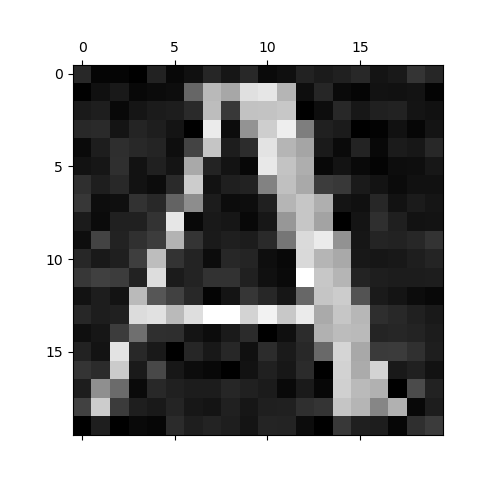
\includegraphics[width=\textwidth]{pictures/A_normalpng.png}
    \caption{Image before HOG.}
    \label{fig:noHOG}
  \end{minipage}
  \hfill
  \begin{minipage}[b]{0.22\textwidth}
    \includegraphics[width=\textwidth]{pictures/A_HOG.png}
    \caption{Image after HOG.}
    \label{fig:HOG}
  \end{minipage}
\end{figure}




\subsection{CNN}

Pre-processing for convolutional networks is executed in layers. Prior to the classification process, the data is reshaped with several techniques including \textit{convolutional, pooling} and \textit{dropout} layers.

% Convolutional layers
A convolutional layer systematically applies learned filters to the input images in order to create feature maps that summarize the presence of those features in the input \cite{Brownlee2019}. The approach is proven to be very effective, and stacking them in deep models allows the layers to learn abstract features like shapes and objects. This is very intuitive for our data, as recognizing line segments and curves are directly applicable for characters. However, the convolutional layers record the position of the features in the input with high precision. This means that even small distortions of the feature in an input image will result in a totally different feature map. Such changes are prone to happen when the input image is noised, shifted or rotated.

% Max pooling
To counteract the limitations of the convolutional layers, a subsequent Maximum pooling layer is added. Pooling helps to make the representation become approximately invariant to small translations of the input  \cite{Brownlee2019}. The layer will summarize the most activated presence of a feature to down-sample the feature map, like in Figure \ref{fig:maxP}. This way, the small movements detected by the convolutional layers will result in a pooled feature map with the feature located in the same place.

\begin{figure}[H]
    \centering
    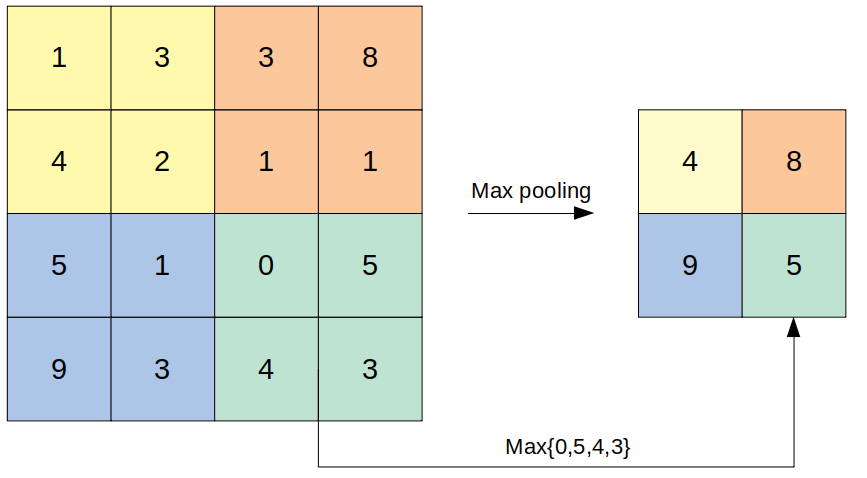
\includegraphics[width=0.45\textwidth]{pictures/maxPooling.png}
    \caption{Max Pooling process.}
    \label{fig:maxP}
\end{figure}

% Dropout to prevent overfitting
For further processing, a dropout layer is included. The dropout technique randomly selects neurons that will be neglected for the duration of the current iteration. It is believed that the network this way will learn multiple independent internal representations \cite{Brownlee2016}. Practically, the layer will drop out randomly selected features. The effect of dropout layers is a reduced chance of \textit{overfitting} as the network becomes less sensitive to specific weights of neurons.



\subsection{ALTERNATIVE TECHNIQUES}

Examining the images of the letters, they seem to be greyscale images where the contour of the letters fits snuggly inside the image frame. Hence, cropping were not a necessary measure, as the letters fit perfectly inside the frame.

The noise layers that can be applied with Keras seems very interesting for this task. Adding noise to a model with a small training dataset can reduce the chance of overfitting. Chars74k-lite has 7112 images in total, yielding 273 images per character which is prior to splitting them in training and test sets. Augmenting the dataset with noised images could prove to make the model more accurate. We did try to supplement the existing dataset with augmented data using a data generator tool from Keras, however it seemed to directly transform the data and not simply append it to our dataset. After completing the full machine learning project did we find a way to extend our dataset with augmented images, which it is not used in our code.

However, a tool from Keras called Data Generators were instead applied, which has the same purpose:  adding flipped, rotated and rescaled images. 

For the SVM we tried to convert to greyscale and apply a blur to remove possible "salt and pepper" noise (misplaced black and white dots), but it only seemed to decrease the accuracy by a few tenths.

Another method that were considered for the SVM was a Principal Component Analysis (PCA). PCA reduces the number of dimensions by projecting them onto a lower-dimensional sub-space \cite{scikit-learn}. For instance it would be possible to produce some kind of projection of the a-z letters onto a 3d plane, by finding the three variables that contains most of the information about the image. It would be cool to maybe try to plot them on a 3d graph, but we deemed it unnecessary.


\section{CHARACTER CLASSIFICATION}
\label{sec:class}

\subsection{Initial thoughts}
% After having looked at the dataset, did you have any initial idea about what kind of model that might work well?  Explain your reasoning.
OCR involves interpreting images and inferring characters. With this in mind, Artificial Neural Networks (ANN's) became a natural choice the task. ANN's excel at performing object recognition tasks. Their popularity have risen dramatically in recent years, partially due to the high accuracy they achieve in tasks that involve computer vision. Especially effective for problems like OCR is the Convolutional Neural Networks (CNN's). The intuition of using a CNN aroused from its very nature: they preserve the spatial relationship between pixels in an image, and use this to extract surprisingly abstract features in their classification process. The networks are also very modular as a large variety of layers can be applied.

To compare with the CNN, we wanted a \textit{simpler} and a less complex method that would provide adequate classification accuracy. We chose to use an SVM, which is widely recognized in classification problems, so there should not be too large of a gap between the models when classifying the letters. A CNN is a non-linear classifier because of its use of non-linear activation functions, whereas an SVM is a linear classifier because it uses kernels to project features onto a hyperplane where it is possible to separate the classes linearly. 

\subsection{Choice of classifiers}
% Give a description of the two models you elected to use. The description must include a brief explanation on how they work. Why did you select these models?
\subsubsection{SVM}
The Scikit implementation of a multiclass SVM uses a "one-vs-one" approach and might look cumbersome when it comes to computational time \cite{sklearn_api}. However, compared to something like k-NN, which must evaluate the dataset every time, we will have a trained model that can be applied easily. The main reason for choosing an SVM was because we wanted to compare it with the CNN algorithm. Before implementation, we hypothesized that the CNN would outperform the SVM, which would not necessarily be true for OCR.

\begin{figure}[H]
    \centering
    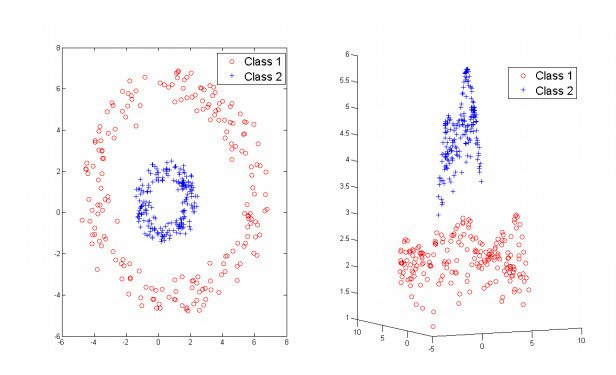
\includegraphics[width=0.45\textwidth]{pictures/SVM.png}
    \caption{The SVM finds a hyperplane (r.h.s.) that makes the classes linearly seperable.}
    \label{fig:SVM}
\end{figure}

SVM is a supervised machine learning algorithm that can be employed for both classification and regression purposes. Basically, SVM finds a hyperplane that divides the dataset (Figure \ref{fig:SVM}). Support vectors are the points nearest to the hyperplane. The hyperplane may be altered if any support vectors are removed from the dataset.

SVM uses different kernels to find the hyperplane. Although the model has auto-tuning, it still relies on an expert to tune the parameters to gain those extra accuracy points. In this experiment it was an easy choice to use the Radial Basis Function (RBF) kernel, also known as a Gaussian Kernel. The RBF kernel has two parameters $\gamma$ (\textit{gamma}) and '$C$'. $\gamma$ is the inverse of the radius of influence of the support vectors and $C$ trades off correct classification of training examples against maximization of the decision function’s margin (hyperplane) \cite{scikit-learn}. Support vectors are the data points samples selected by the model closest to the separation boundary between the classes on the hyperplane axis. 

To find a optimal parameter selection for this kernel, we cross-validated different combinations that were pipelined into the "GridSearchCV" method provided by sklearn. A grid search performs hyper parameter tuning in order to find the best possible values for a given model. This can make a significant difference for a SVM model. The grid searched through the following parameters:
\begin{lstlisting}[language=Python]
parameters = {
    'clf__gamma': (0.1,0.25,0.5,1,1.5),
    'clf__C':     (1,1.5,2,2.5,3,2.5),
}   
\end{lstlisting}
and found the best parameter combination for the RBF kernel to be $C=3$ and $\gamma=1$.



\subsubsection{CNN}
A convolutional neural network is a class of deep neural networks that specializes in feature extraction and processing data with a grid-like topology, e.g. image data. A variety of filters are used to reveal characteristics of the input. In the first layers these characteristics can be lines or circles, while in deeper layers they can form abstract objects like faces. Compared to conventional deep neural networks, CNN's store fewer parameters which reduce the memory requirements and improve the statistical efficiency. 

In its essence, a CNN has three types of layers: convolutional layers, pooling layers and dense layers \cite{Brownlee2019a}. An example showing these layers is depicted in Figure \ref{fig:cnn}. The convolutional layers are compromised of filters and feature maps. Their task is to extract features from the input. A pooling layer follow a sequence of one or more convolutional layers, and are intended to consolidate the features learned in the features maps. In other words, it is meant to compress or generalize feature representations and thus reduce the chance of overfitting the model. Lastly, the dense layers are included at the end of the network, after feature extraction and consolidation, to create final non-linear combinations of features and make predictions. 

\begin{figure}[H]
    \centering
    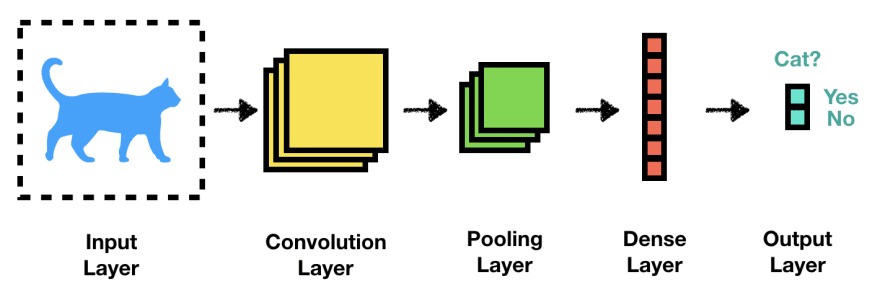
\includegraphics[width=0.45\textwidth]{pictures/cnn.png}
    \caption{Representation of the layered structure in a convolutional neural network.}
    \label{fig:cnn}
\end{figure}

\subsection{Evaluation of the classifiers}
% A critical evaluation of your two models.  
% How are you measuring their performance?  
% How did they do?  
% Which model gave the best results?  
% Include at least five predictions in the report (both good and bad).


Performance of the CNN is measured when the trained model is evaluated with the test samples. In Keras, there is a function called \verb|evaluate()| that outputs the test loss and test accuracy. The SVM accuracy was obtained by creating a function that cross-validates the predictions of the test-set with their real value. The common performance measure for the two models will therefore be the accuracy.

Figure \ref{fig:accSVM} and \ref{fig:accCNN} displays some samples from the classification process with SVM and CNN, respectively. Above each image, both the true label and the prediction is given. Looking at nine random predictions made by the models, which has an accuracy of about 80-90\%, at least one of the predictions should be a wrong classification. The prediction in the upper left corner of figure \ref{fig:accSVM} is an example of a faulty prediction. If we were to speculate, it might be that the dataset contains more lower-case \textit{t}'s rather than upper-cases (\textit{T}), and the opposite is true for an \textit{i}. On the other side, the image is very blurry, which might have been preventable by supplementing the training data with blurred copies of the original data. Another bad prediction can be seen by the prediction in the upper right and lower left corner of the CNN predictions in figure \ref{fig:accCNN}. The lower left "i" was predicted as a "l", which is understandable given that bottom of the next letter in the image will trick the CNN into thinking that these pixels are more likely connected.

\begin{figure}[H]
    \centering
    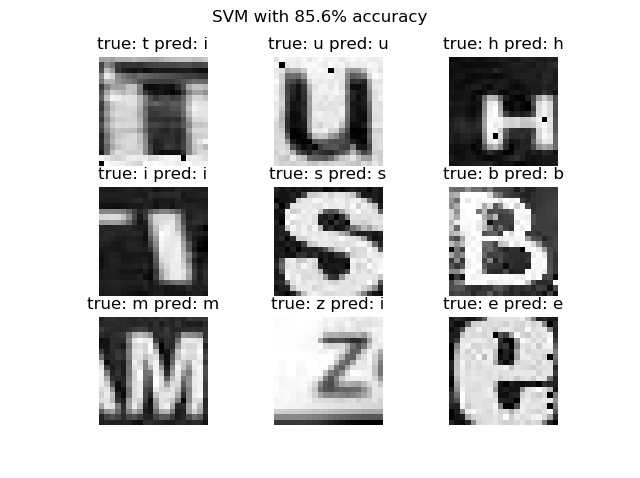
\includegraphics[width=0.45\textwidth]{pictures/accSVM.png}
    \caption{Samples from the classification process with SVM.}
    \label{fig:accSVM}
\end{figure}

\begin{figure}[H]
    \centering
    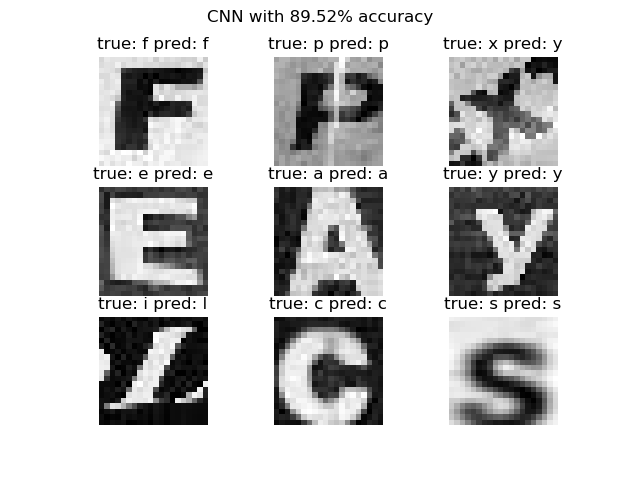
\includegraphics[width=0.45\textwidth]{pictures/accCNN.png}
    \caption{Samples from the classification process with CNN.}
    \label{fig:accCNN}
\end{figure}

As it can be seen from the samples above, both models achieved a good accuracy. However, the overall highest accuracy was as expected accomplished by CNN with \textasciitilde 89\%, as to \textasciitilde 85\% for the SVM.

\subsection{Alternative classifiers}
% Were there any additional models that you would have liked to try, but for some reason were notable to?  Explain.

It would be interesting to test the k-Nearest Neighbour (k-NN) algorithm for character classification. It would be fun to know the accuracy of such a straightforward and humble algorithm. The k-NN algorithm would probably work best if we performed some of the same pre-processing steps as for the SVM, such as converting to gray-scale (potentially binary) and extracting the HOG.

Another method we could have implemented for this project is ensemble methods, which use various learning algorithms to obtain a better prediction than the models would get individually. Aggregating a diverse set of models into one would make it more robust and able to handle new data much better. We could have, for instance, combined the result of both of our methods to produce a more favorable result. 





\section{CHARACTER DETECTION}

For the last endeavor of this project, we are to detect and predict letters in an image with the help of object detection or object localization. We were able to do so with the help of our classifiers and a technique called \textit{sliding window}. The idea behind a sliding window is to divide a larger image into smaller windows of fixed size and apply an image classifier to determine if a target is in the picture - in our case a letter. We implemented a simple adjustable sliding window for each of the algorithms, which returns an image with green squares around a \textit{valid} classification while printing the letter.

\subsection{Detection}
% Test your character detector on detection-1.jpg and detection-2.jpg and show the result in the report.  Feel free to find or create additional images to test your detector, if you are so inclined.
The parameters for the following two detection images were kept the same: the step size was kept at 4, i.e. it moves 4 pixels per window, and the window size was 20x20.

\subsubsection{detection-1.jpg}
Both methods were capable of detecting all letters, but apparently struggled with the 'S' . The sliding windows whose classification had a confidence level higher than the probability threshold set in the algorithm are shown as green squares in Figure \ref{fig:svm_detect}. To be able to classify the 'S', the confidence boundary of both algorithms were reduced to \textasciitilde 88\%, which is why a second 'E' is classified (if you look closely).

\begin{figure}[H]
    \centering
    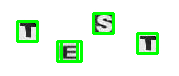
\includegraphics[width=0.2\textwidth]{pictures/svm_pred.png}
    \caption{"T-E-S-T"}
    \label{fig:svm_detect}
\end{figure}

\subsubsection{detection-2.jpg}

The second image (figure \ref{fig:svm_detect2}) was predicted by the CNN model. The performance was not satisfactory at all and there are a few things we could have done differently, which will be discussed in the evaluation of this section. There seemed to be a problem with the confidence of our Keras CNN models, as it was almost always above 99.9\% sure about its classifications, which made it hard to decide on a confidence threshold and partly explains all the redundant squares. The model had ~65\% accuracy in the classifications made in the image.


\begin{figure}[H]
    \centering
    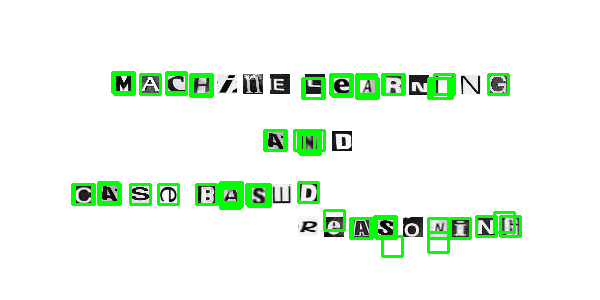
\includegraphics[width=0.5\textwidth]{pictures/svm_pred2.png}
    \caption{"MACHINE LEARNING AND CASE BASED REASONING"}
    \label{fig:svm_detect2}
\end{figure}

\subsection{Evaluation and potential improvements}
% Give an evaluation of your detection system.  How does it perform?
% Describe any improvements you made to your detector.  Discuss how you can improve your system further.

Our detection algorithms performed well on the first image and not so good on the second, but it has a lot of potential. The first giveaway is that the required confidence level that were used could be lower in order to detect the more obscure letters. We could have reduced it if we implemented a restriction to the re-classification of the same letters in windows close to each other. A simple votation or average confidence between of the neighboring windows was considered, as well as removing outliers such as all-white images. An average of neighbors would also reduce the possibility of a faulty classification.

Another improvement we could have tried is to use different representations of the image and the sliding windows. Characters could have different orientations, and different angles and projections of the image/window should be evaluated and consider as possible classifications. 

Every possible scale of the image could also be considered. One possible way to do this is to use "\textit{Image Pyramids}", which is a multi-scale representation of an image. This would help our sliding window by making it able to classify characters that require smaller scales.

In the second detection image (figure \ref{fig:svm_detect2}) there was a lot more obscure characters and some with different orientations. As we mentioned, this could have been accounted for if we had extended our dataset with augmented representations of the existing samples.

\section{CONCLUSION}

% What is the weakest and strongest component of your OCR system (feature engineering, character classification, and character detection)?  Explain your answer.


% What went good/bad with the project?  Any lessons learned?

With the existence of open source and an abundance of machine learning tools, you do not need a degree in computer science to perform machine learning. You should, however, know what type of model to apply to a given problem, and the features are more likely to make the model more capable of discriminating between different classes. This project introduced us to a lot of new models and methods of performing machine learning, which has led to in-depth investigations of documentation and tutorials in order to produce the most successful algorithm. When using existing and well-tested libraries like Keras and Sklearn, a large portion of the effort is to read and understand other's work. For instance, it was helpful to have a basic understanding of how a neural network works, but the process of implementing a CNN in this assignment gave a more profound understanding of how different parts of a neural network can be tweaked to alter the result, based on the area of application.

Much time was used trying to improve the accuracy of the classifiers in Section \ref{sec:class}. With little knowledge of how the training process works, tendencies towards brute force had little effect on the results. Even though we trained and tested multiple generations of models with different hyperparameters, it seemed like most of the model's performance depended on correct preprocessing of the data. Applying and knowing what feature's and how it is fed to the ML model will be of much higher importance the next time we are to set up a pipeline for a machine learning problem.

\printbibliography[title={REFERENCES}]

\end{document}